%!TEX root = ../main.tex

\documentclass[../main.tex]{subfiles}
\begin{document}

\chapter{Introduction}
\label{chapter:introduction}

Our reliance on robots to keep our society functioning is increasing. As time goes on, more and more industries face changes in the technology landscape where the utilization of robots becomes a financial inevitability. This phenomenon drives the innovation that leads to smarter, cheaper, and more reliable robots. The proliferation of robots seems to fuel the automation of our daily lives where any task with minor repetitiveness is subject to automation. Some tasks like driving a car on the road or winning a game of Go, which were thought to be solvable only by humans, are already performed by computers equipped with some form of Artificial Intelligence. However, there are still a number of tasks that do not have satisfiable automated solutions. These tasks vary from safety critical tasks that directly impact lives to business operations tasks that determine profitability and efficiency of an organization.

Some examples of high impact tasks include search and rescue in the wilderness, natural disaster monitoring and relief, demining, and surveillance. Some examples of operations tasks are floor sweeping, factory automated painting, crop health monitoring, and ship hull inspection. The types of applications are broad but they all share a common theme. In fact, in its most general form, the problems described so far could all be stated as a coverage path planning problem.

The coverage path planing problem is a problem of computing a path for a robot such that the traversal of that path by the robot results in all points in the environment being under the robot's footprint as some point of time during the traversal. An example of a robot performing a coverage task is shown in Figure~\ref{img:example_coverage}. The problem is as old as the machine controlled milling. Only in 2000, Arkin\cite{arkin2000approximation} has demonstrated that the problem is in fact NP-complete. As such, there are numerous suboptimal solutions that have been proposed over the years. There are two surveys by Choset~\cite{choset2000coverage} and Galceran~\cite{galceran2013survey} that outline the most accepted solutions. Moreover, there is an extension to this problem that has been gaining popularity over the recent years. The use of multi robot systems for coverage to achieve better performance is becoming more appealing caused by decreasing cost of building robots.

\begin{figure}[]
	\centering
	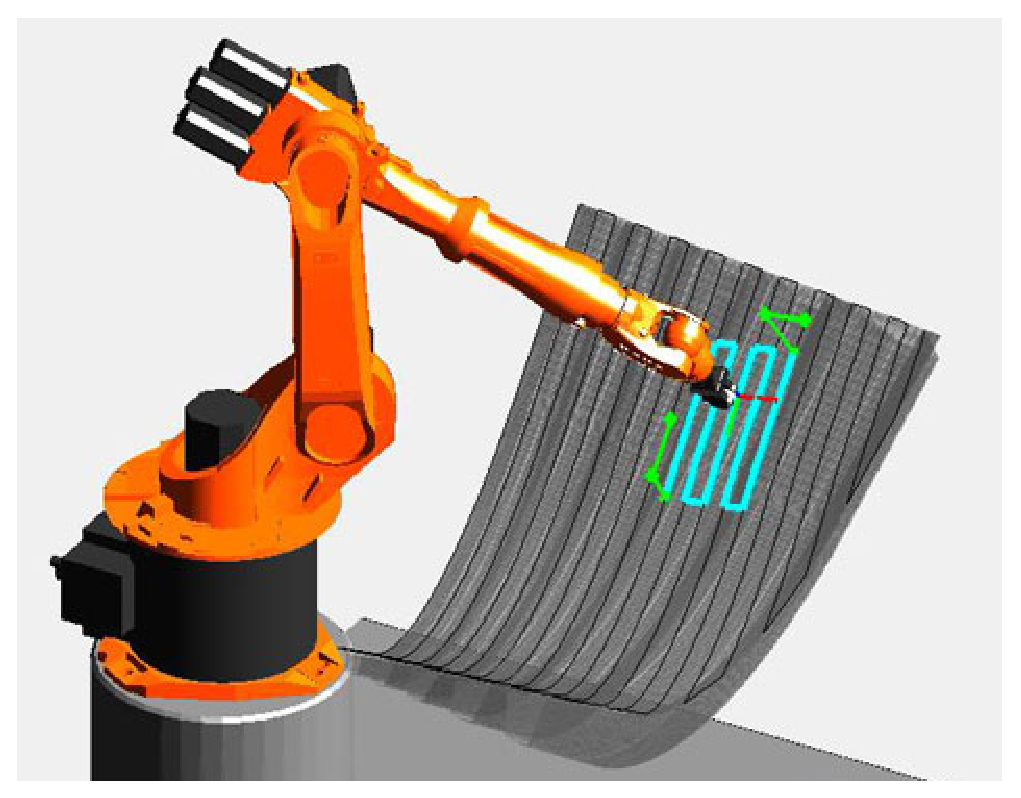
\includegraphics[scale=0.5]{img/chapter_1/example_coverage.eps}
	\vskip-15pt
	\caption*{\tiny twi-global.com}
	\caption{An example of an inspection coverage performed by a robotic arm.}
	\label{img:example_coverage}
\end{figure}

It is difficult to think about a good solution to the coverage path planning problem because the notion of \emph{goodness} varies from one application to another. For example, a good coverage path for a painting robot would result in the most uniform paint layer on the surface. A good coverage path for a monitoring application would result in the entire area observed in high quality. Because of this variety of metrics, the existing solutions in literature are typically very specialized. Other works in literature that focus on the theoretical analysis of the problem propose solutions that theoretically achieve complete coverage but in practice, are not feasible for any robot with the simplest of dynamics.

In this work, we propose an approach that aims to make coverage paths more usable in practice. We do this by structuring the paths generated by our method to be as \emph{straight} as possible. This is motivated by the typical dynamics of robots. Straight line segments are the simplest path segments that a robot can traverse. Vast majority of robotic systems are designed in a way that the traversal of a path between point $A$ and $B$ is the most efficient when this path is a straight line. In other words, we aim to compute paths with minimum number of turns. It should be noted that this goal can be achieved by minimizing the number of straight line segments required for complete coverage since every straight line segment has a turn associated with it to transition to the next straight line segment.

Our main contributions in this work are several. First, we design our own metric called the altitude that aids with the computation of the number of lines for full coverage. We then propose a greedy algorithm that partitions the workspace into regions with the minimum overall altitude. The result of the algorithm is a workspace partition with a set of lines. One of the important aspects of the algorithm is the procedure to make a minimum altitude cut dividing a polygon into two. We then solve the coverage problem by planning a tour of straight line segments by framing the problem is a Generalized Traveling Salesman Problem. We also provide proof of correctness of the algorithm as well the computational complexity analysis. Our final contribution is the extension of the single-agent coverage to the multi-agent case. We propose a partitioning scheme that divides the workspace into regions that results in comparable amount of work for each robot. The single robot coverage is then solved for each robot in the partition. 

\end{document}